% Created 2024-10-21 Mon 00:24
% Intended LaTeX compiler: pdflatex
\documentclass[12pt]{article}
\usepackage[utf8]{inputenc}
\usepackage[T1]{fontenc}
\usepackage{graphicx}
\usepackage{longtable}
\usepackage{wrapfig}
\usepackage{rotating}
\usepackage[normalem]{ulem}
\usepackage{amsmath}
\usepackage{amssymb}
\usepackage{capt-of}
\usepackage{hyperref}
\usepackage[margin=1in]{geometry} \usepackage{amsmath}
\author{Jason Press}
\date{\today}
\title{Friction in Atwood Machines}
\hypersetup{
 pdfauthor={Jason Press},
 pdftitle={Friction in Atwood Machines},
 pdfkeywords={},
 pdfsubject={},
 pdfcreator={Emacs 29.4 (Org mode 9.7.11)}, 
 pdflang={English}}
\begin{document}

\maketitle
\begin{abstract}


In this lab, we determined the amount of work friction did in two different Atwood machines, along with the mechanical advantage of both Atwood machines. The first Atwood machine we tested was the standard single pulley Atwood machine, with two masses suspended by a string around a pulley. Using the Work-Energy Theorem, we determined that friction did \(-0.00634 \pm 0.00206\)J of work in this system. Using a spring scale, we determined the mechanical advantage of the single pulley to be 1. The second Atwood machine we tested was a double pulley Atwood machine, where the line was attached to the ceiling, then a pulley holding the first mass, then the Atwood pulley, then the second mass. Using the Work-Energy Theorem, we determined that friction did \(-0.107 \pm 0.079\)J of work in this system. Using a spring scale, we determined the mechanical advantage of the system to be 2.
\end{abstract}
\section{Introduction}
\label{sec:org6f9b124}

In this lab, we used the Work-Energy Theorem to determine how much energy friction leeched from two different Atwood machine systems. Additionally, we determined the mechanical advantage of the two different Atwood machine systems. The first Atwood machine was the standard one pulley system, with two masses connected by a pulley. The second Atwood machine was a two pulley system, with the first mass connected to a second pulley.

To calculate the work done by non-conservative forces (friction), we can use the Work-Energy Theorem to describe how much energy is lost due to friction:

\begin{align*}
W_{NC} = \Delta K + \Delta U = (K_f - K_i) + (U_f - U_i)
\end{align*}

Then, assuming the system has no initial kinetic (the system starts at rest) nor potential (an arbitrary choice to make calculations easier, since we can dictate what \(U_i\) is) energy, and using \(\bar{v} = \frac{v_i - v_{f}}{2} = \frac{h}{t} \implies v_f = \frac{2h}{t}\), we get the equation for describing the work done by non-conservative forces in a single pulley Atwood machine:

\begin{align}\label{eq:single}
W_{NC} = 2 \left( \frac{h}{t} \right)^2 (m_1 + m_2) + g h (m_1 - m_2)
\end{align}

Similarly, for the two pulley system, we get the following equation, knowing that \(h \equiv \frac{h_{m_2}}{2} = h_{m_1}\):

\begin{align}\label{eq:double}
W_{NC} = 2 \left( \frac{h}{t} \right)^2 (m_1 + 4 m_2) + g h (m_1 - 2 m_2)
\end{align}

We assumed all of the work done by non-conservative forces \(W_{NC}\) to be done by friction.

To determine the mechanical advantage of a system, we simply evaluated \(\frac{\text{force out}}{\text{force in}}\).
\section{Methods}
\label{sec:org4ee3396}

For the single pulley system, we suspended one pulley from a mounting point on the ceiling. Then, we threaded a fishing line through the pulley and attached it to two mass hangers of equal weight (\(w = 50g\)). For the mass we wanted to go down, \(m_2\), we added an additional 4g. We used enough line so that \(m_2\) would make contact with the table, while ensuring there was enough line for \(m_1\) to travel vertically without hitting the pulley.

For the double pulley system, we kept the single pulley from a mounting point on the ceiling, but also attached one end of the line to the ceiling. Then, we added a pulley to \(m_1\). We threaded the free end of the line through the \(m_1\) pulley, then through the mounted pulley, then attached it to \(m_2\). Again, we positioned the pulley such that \(m_2\) would travel down to the table, and ensured that both masses could travel freely between the starting point and the ending point. We placed enough mass on \(m_2\) so it would travel down. After we ran the trials, we weighed \(m_1\) with the pulley because the mass of the pulley was unknown.

In order to evaluate Equations \ref{eq:single} and \ref{eq:double}, we needed to experimentally determine two values, \(h\) and \(t\).

To obtain \(h\) for each trial, we put the bottoms of \(m_1\) and \(m_2\) at the same level, \(h = 0\). Since both masses move the same distance in the single pulley system and \(m_2\) moves twice as much as \(m_1\) in the double pulley system, we can measure the height \(m_2\) travels as the distance from the base of \(m_2\) at \(h = 0\) to the resting place of \(m_2\), and then deduce the distance \(m_1\) travels knowing the distance \(m_2\) travels. We placed a meterstick with the zero mark on the table, and recorded the height of \(m_2\) when both masses were at \(h = 0\) to determine \(h_2\).

To obtain \(t\) for each trial, we used a stopwatch. We counted down when to release both masses to ensure the masses were released the instant the stopwatch started, and stopped the stopwatch when \(m_2\) hit the table.

For both experiments, we did \(N = 10\) trials to minimize statistical error.

To obtain the mechanical advantage of the system, we placed a 500g weight on \(m_1\), and attached a spring scale on \(m_2\). Then, we held the free end of the spring scale still, and when the system reached an equilibrium, we read the measurement of the spring scale. \(m_1\) was force in, and \(m_2\) was force out.

\begin{center}
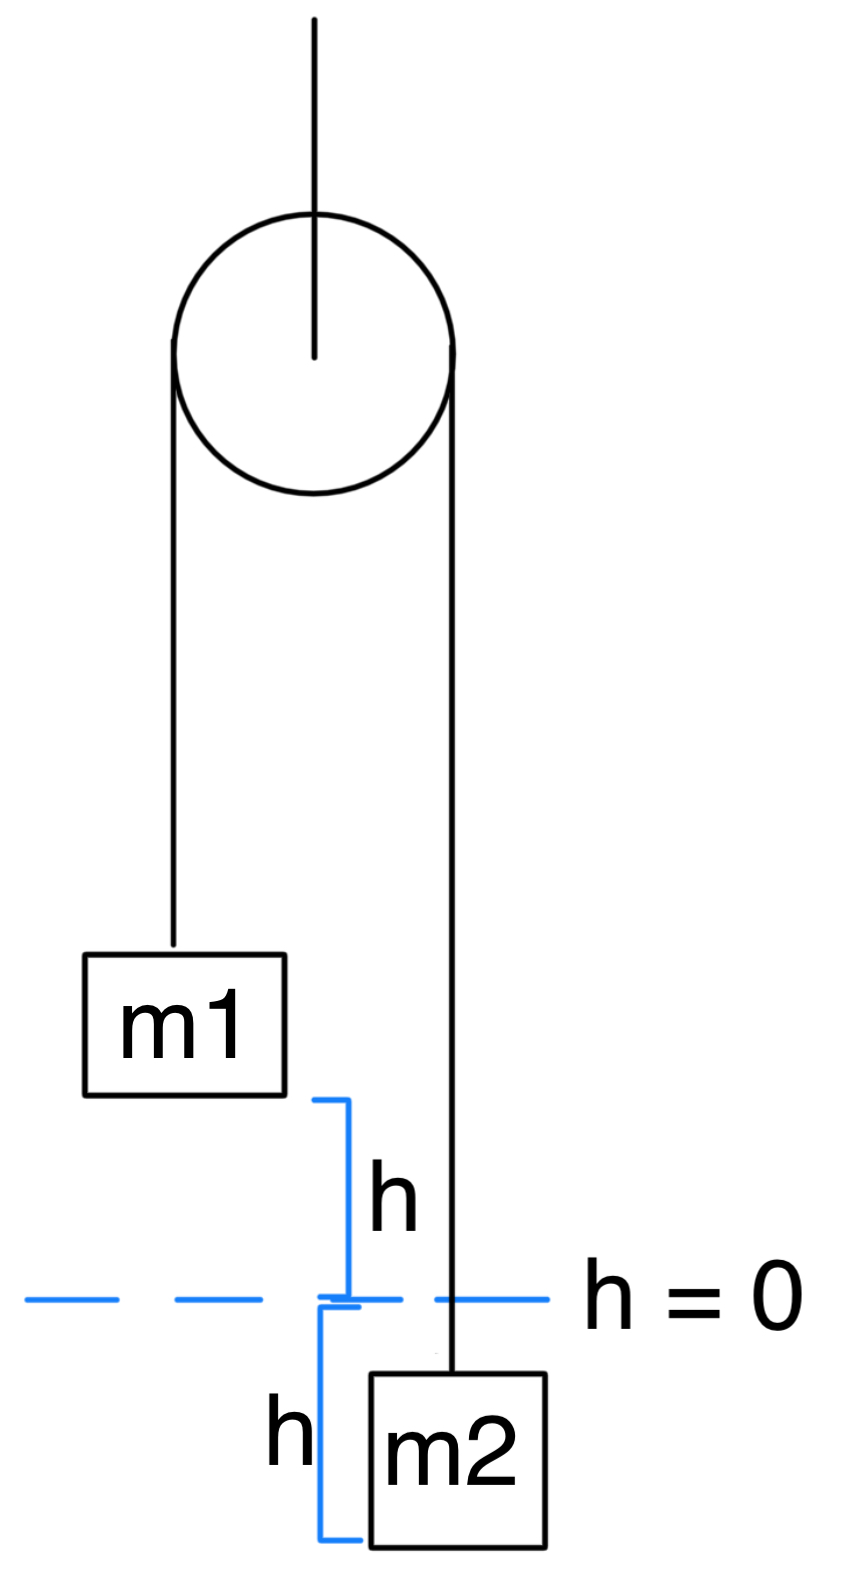
\includegraphics[height=4in]{./singlepulley.png}
\captionof{figure}{Single pulley system}
\end{center}

\begin{center}
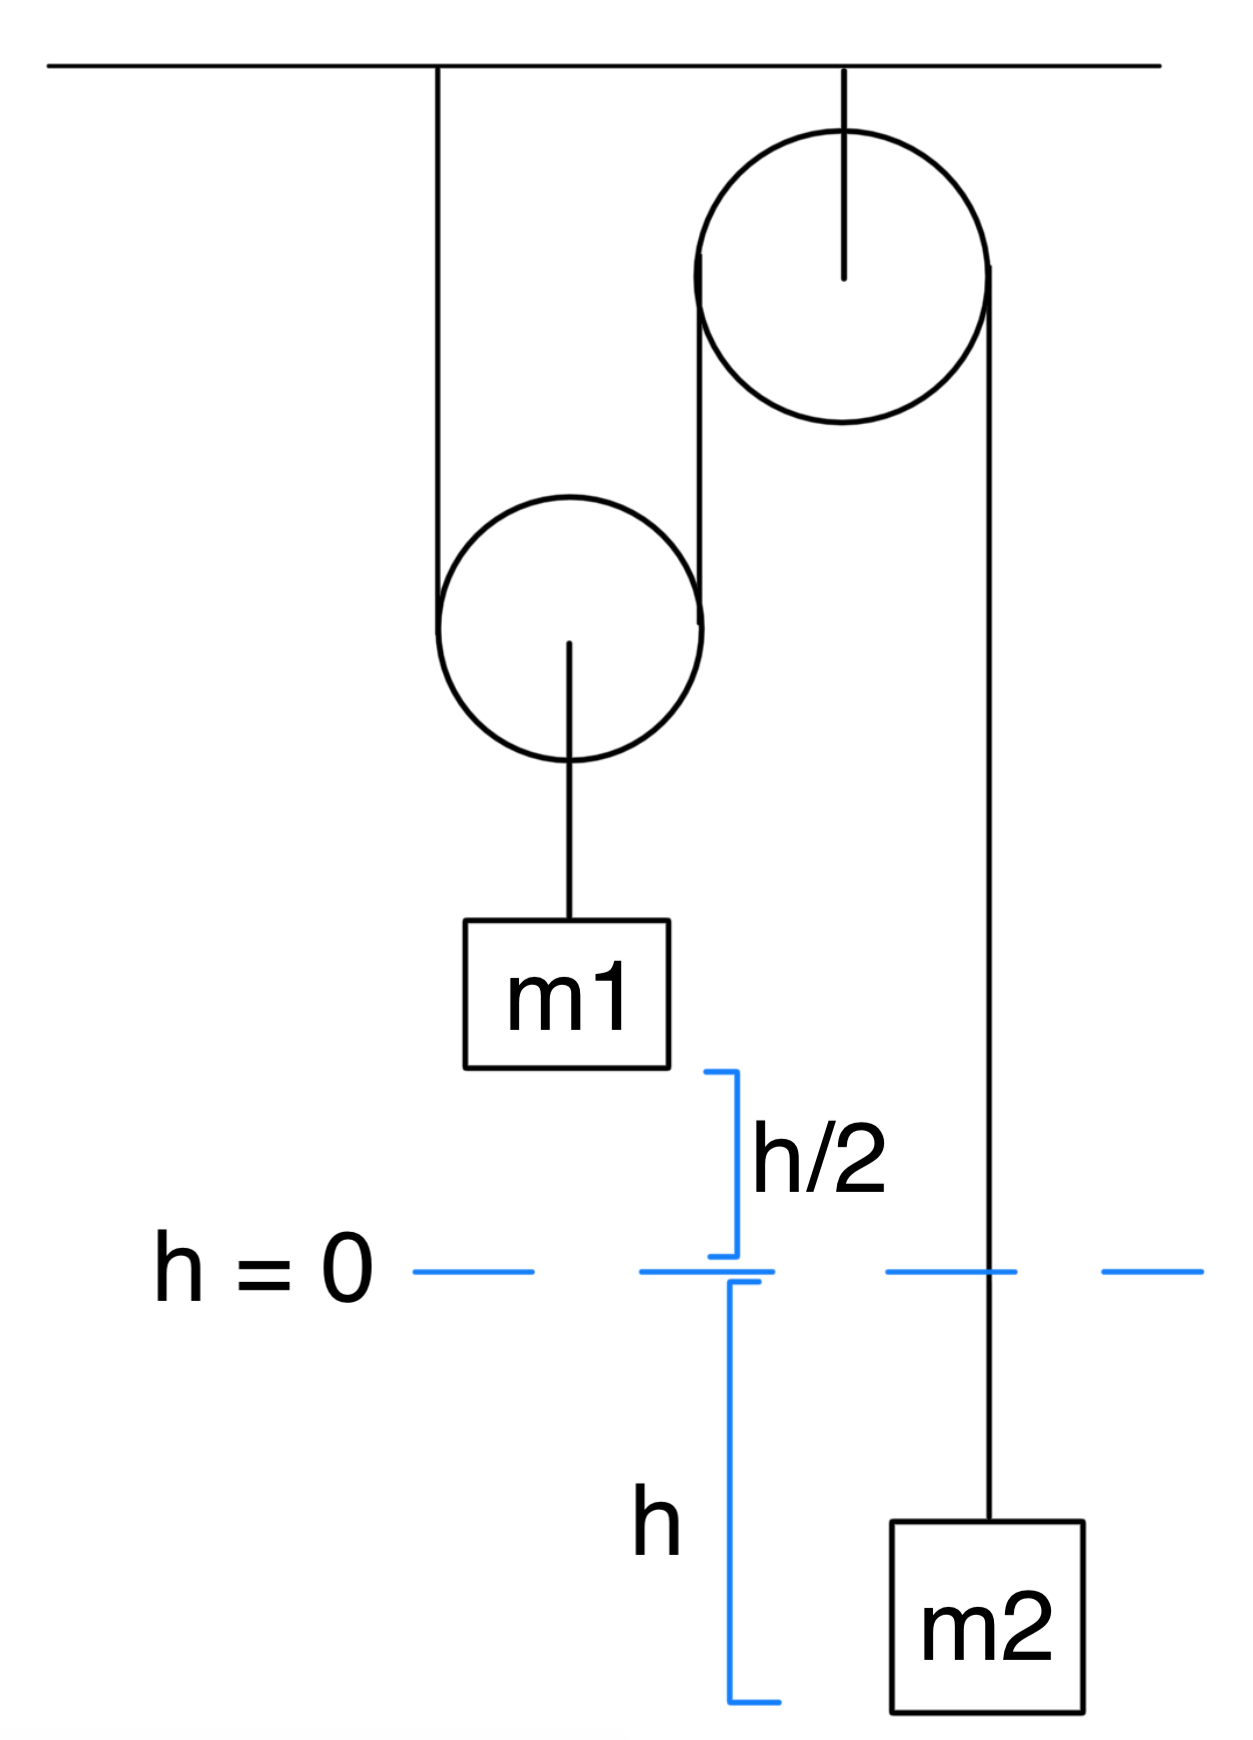
\includegraphics[height=4in]{./doublepulley.png}
\captionof{figure}{Double pulley system}
\end{center}
\section{Results}
\label{sec:org8cb774f}

Here are our results for the single pulley Atwood machine, with 50g on \(m_1\) and 54g on \(m_2\):

\begin{center}
\captionof{table}{Single Pulley Atwood Machine Results}
\begin{tabular}{r|r|r}
Trial & Height (cm) & Time (s)\\
\hline
1 & 36.5 & 1.86\\
2 & 36.5 & 1.88\\
3 & 36.5 & 1.58\\
4 & 36.6 & 1.76\\
5 & 36.6 & 1.83\\
6 & 36.6 & 2.08\\
7 & 36.5 & 1.91\\
8 & 36.6 & 1.94\\
9 & 36.6 & 2.06\\
10 & 36.5 & 1.74\\
\hline
Average & 36.55 & 1.864\\
\end{tabular}
\end{center}

Using Formula \ref{eq:single}, we get \(-0.00634 \pm 0.00201\)J of work due to friction. Additionally, the mechanical advantage of the system was 1: when we put 550g on \(m_1\) and a spring scale on \(m_2\), the spring scale read 550g of force.

Here are our results for the double pulley Atwood machine, with 96.6g on \(m_1\) and 80g on \(m_2\):

\begin{center}
\captionof{table}{Single Pulley Atwood Machine Results}
\begin{tabular}{r|r|r}
Trial & Height (cm) & Time (s)\\
\hline
1 & 38.7 & 1.34\\
2 & 38.6 & 1.56\\
3 & 38.8 & 1.69\\
4 & 38.9 & 1.73\\
5 & 38.6 & 1.41\\
6 & 38.7 & 1.59\\
7 & 38.8 & 1.49\\
8 & 39.1 & 1.63\\
9 & 38.7 & 1.69\\
10 & 38.7 & 1.4\\
\hline
Average & 38.76 & 1.553\\
\(h \equiv h_{m_1} = \frac{h_{2}}{2}\) & 19.38 & N/A\\
\end{tabular}
\end{center}

Using Formula \ref{eq:double}, we get \(-0.107 \pm 0.004\)J of work due to friction. Additionally, the mechanical advantage of the system was 2: when we put 600g on \(m_1\) and a spring scale on \(m_2\), the spring scale read 300g of force.
\section{Discussion}
\label{sec:orga096833}

To determine the error, we used the standard formula for error prorogation in a system to obtain the error for the single pulley system:

\begin{align}
\sigma^2 = \left( \frac{(-4 h^2 (m_1 + m_2))}{t^3} \right)^2 \sigma_t^2 + \left( g (m_1 - m_2) + \frac{(4 h (m_1 + m_2))}{t^2} \right) ^2 \sigma_h^2
\end{align}

And derived a similar equation for the two pulley system:

\begin{align}
\sigma^2 = \left( \frac{(-4 h^2 (m_1 + 4 m_2))}{t^3} \right) ^2 \sigma_t^2 + \left( g (m_1 - 2 m_2) + \frac{(4 h (m[1] + 4 m[2]))}{t^2} \right)^2 \sigma_h^2
\end{align}

And \(\sigma_h\) and \(sigma_t\) in each system is the square root of the sum of squares of their respective statistical systematic, and resolution errors.

The overall amount of work done by friction was small. In the single pulley system, \(m_1\) did -0.175J of work, while \(m_2\) did 0.200J of work (\(m_1\) did negative work because it was opposing gravity). Relative to the absolute amount of work done by both masses, friction did not perform a lot of work. Similarly, in the double pulley system, \(m_1\) did -0.180J of work, while \(m_2\) did 0.314J of work. Relative to the absolute amount of work done by both masses, friction did not perform a lot of work. However, friction did more relative work in the second system. This was observed with more squeaking noises and a rougher descent of the masses throughout the trials.

For the statistical error, we used the formula for standard error \(SE = \sqrt{\frac{avg}{N}}\). For the resolution error, we used half of the minimum resolution of the respective measuring instrument. For the systematic error for \(h\), we used the resolution error, since our measurements were within half of a division of the meterstick. For the systematic error of \(t\), we used the average reaction time of a human being, 200ms, or 0.2s, since although the mass hits the ground at a predictable time interval, there is an element of reacting to the instant the mass hits the ground.

The mechanical advantage of the single pulley system being 1 makes sense, since the single pulley simply redirects the force of \(m_1\). For the double pulley system, the mechanical advantage of 2 comes from the second pulley being attached to \(m_1\). Although the mechanical advantage of the system is 2, the trade off is that \(m_2\) has to travel twice as far: any advantage in force is compensated with distance. Since \(F = W \cdot d\) for a constant \(F\), a mechanical advantage of 2 means that \(W\) can be \(\frac{1}{2}\), but \(d\) has to be 2 to produce the same \(F\).

This is also observed with how much work both masses do in the second system. By Newton's Second Law, both pulleys experience the same amount of force. However, since \(m_1\) travels half the distance that \(m_2\) travels, \(m_1\) does roughly half of the amount of work that \(m_2\) does (it's not exactly half, since some work is lost due to friction).
\section{Sample Calculations}
\label{sec:orge707679}

We used a spreadsheet for our calculations. To get the average of a column of observations, we used \texttt{=AVERAGE(C2:C11)}. Since we measured \(h\) in cm, and our equations use m, we converted h into m in its own column. To get the work done by friction in a system, we used \texttt{=2*(C13/D12)\textasciicircum{}2*(B4+A4)+9.81*C13*(B4-A4)}. To get the statistical error, we used \texttt{=sqrt(stdev(F2:F11)/10)}. To get the error of a measurement, we used \texttt{=sqrt(C20\textasciicircum{}2+C19\textasciicircum{}2+C18\textasciicircum{}2)}. To get the errors, we broke down each error equation into its components:

\begin{itemize}
\item \verb|=(4*C13/D12^2*(A4+B4)+9.81*(B4-A4))^2*C21^2| for \(\frac{\partial W}{\partial h}^2 \sigma_h^{2}\) and
\item \verb|=(-4*C13^2/D12^3*(B4+A4))^2*D21^2| for \(\frac{\partial W}{\partial t}^{2} \sigma_t^{2}\) in the single pulley system; and
\item \verb|=(4*I13/J12^2*(G3+4*H3)+9.81*(G3-2*H3))^2*I21^2| for \(\frac{\partial W}{\partial h}^{2} \sigma_h^{2}\) and
\item \verb|=(-4*I13^2/J12^3*(G3+4))^2*J21^2| for \(\frac{\partial W}{\partial t}^{2} \sigma_t^{2}\) in the double pulley system.
\end{itemize}
To get the overall error, we took the root of the sum of partials \texttt{=sqrt(C24+C23)}.

For the part in the discussion where I discuss the work done by each mass, we determined the amount of work each mass did with

\begin{itemize}
\item \verb|=1/2*A4*(2*C13/D12)^2+A4*9.81*C13| for \(m_1\) and
\item \verb|=1/2*B4*(2*C13/D12)^2-B4*9.81*C13| for \(m_2\)
\end{itemize}

in their respective system.

For mechanical advantage, we just used \(\frac{\text{mass on }m_1}{\text{scale reading on }m_2}\).

Columns A-F are for the single pulley system, and columns G-L are for the two pulley system. Here is a copy of the spreadsheet we used:

\begin{center}
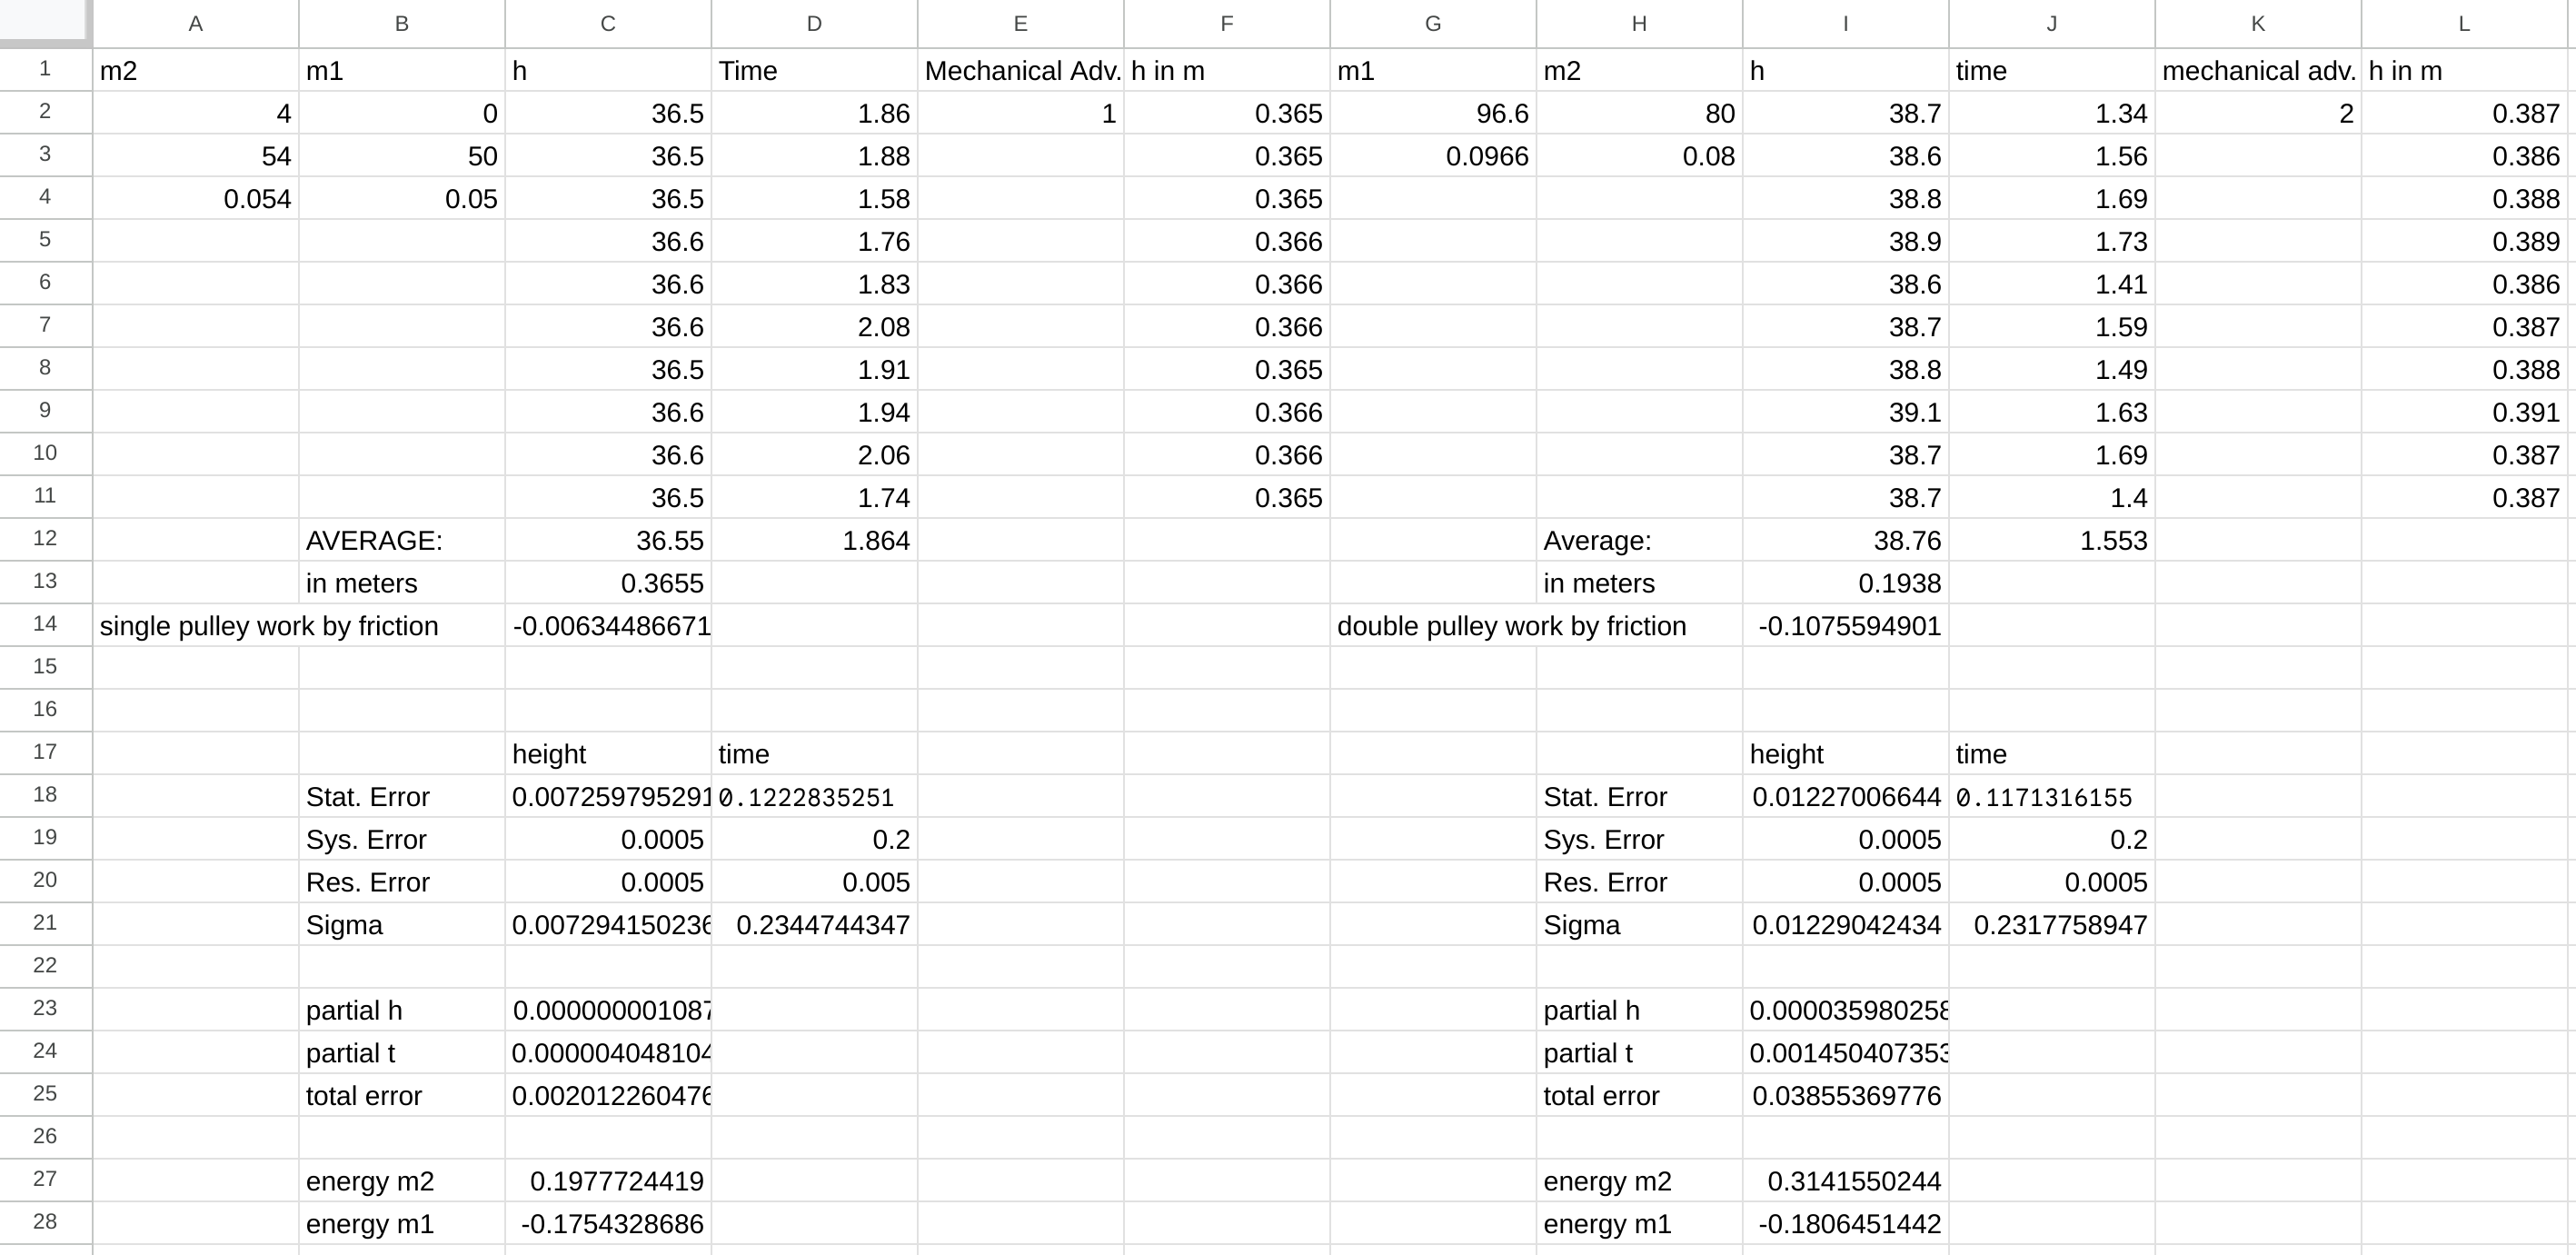
\includegraphics[width=6.5in]{./spreadsheet.png}
\end{center}
\end{document}
